% !TEX root =../thesis-letomes.tex

\chapter{Results}
The main aim of the project was twofold: to examine whether or not ES was a reasonable method to apply in this problem space, and to create a mars mission simulator to compare it with the lunar case, under the expectation that the two problems would be more or less similar. We have accomplished both these things, certainly, even though they did not take the shape we were initially expecting. In this chapter we will examine the various threads of the project, to see where they ended up.

\section{2D Simulator: Effectiveness of Evolution Strategies For This Problem Space}
We implemented several versions of the fundamental ES concept, with different combinations of additions that have given good results in the literature. Certain additions had more impact than others, but no matter what variation we used, the results weren't exactly earth-shattering. The problem space has a fractured, fractal quality of very good solutions hiding among very bad ones. These solutions are not found in any particularly ingenious fashion by ES, nor by any gradient descent method, really. There are areas of good structure, where ES finds a local minimum just fine, but if the objective is simply to find a decent solution, then something naive like random guessing will also perform well, since the space is sufficiently dense with decent solutions. 

When we computed the problem space flattened to two dimensions by locking the burn-angle to 0, we gained valuable information and intuition about its shape. We are dealing with a heavily fractal space of ridges with a cross section of the approximate shape shown in \cref{fig:ridge_cross_section}

\begin{figure}[ht]
    \centering
    \subfloat[The approximate cross-section of the ridges]{
        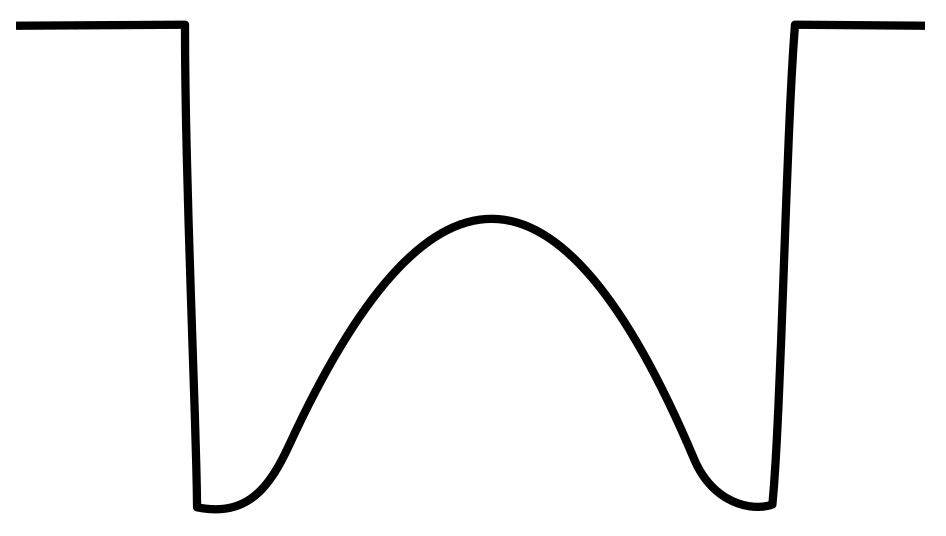
\includegraphics[width=0.46\linewidth]{fig/ridge_cross_section.png}
        \label{fig:ridge_cross_section}
    }
    \hfill
    \subfloat[a ridge in the problem space]{
        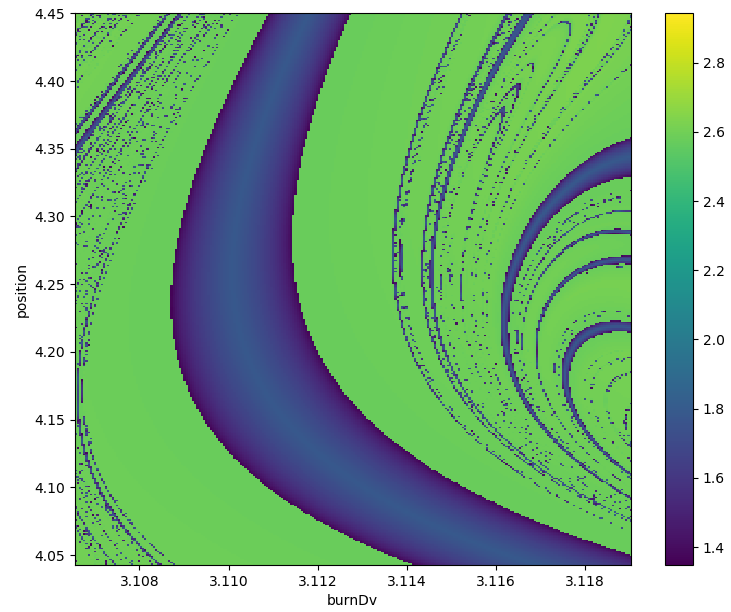
\includegraphics[width=0.46\linewidth]{fig/ridge.png}
        \label{fig:ridge}
    }
    \caption{The problem space is populated densely by ridges with the approximate cross-section seen in \cref{fig:ridge_cross_section}. There are infinitely many of these, if we extrapolate from what we have seen as we have zoomed in.}
\end{figure}

\begin{figure}[ht]
    \centering
    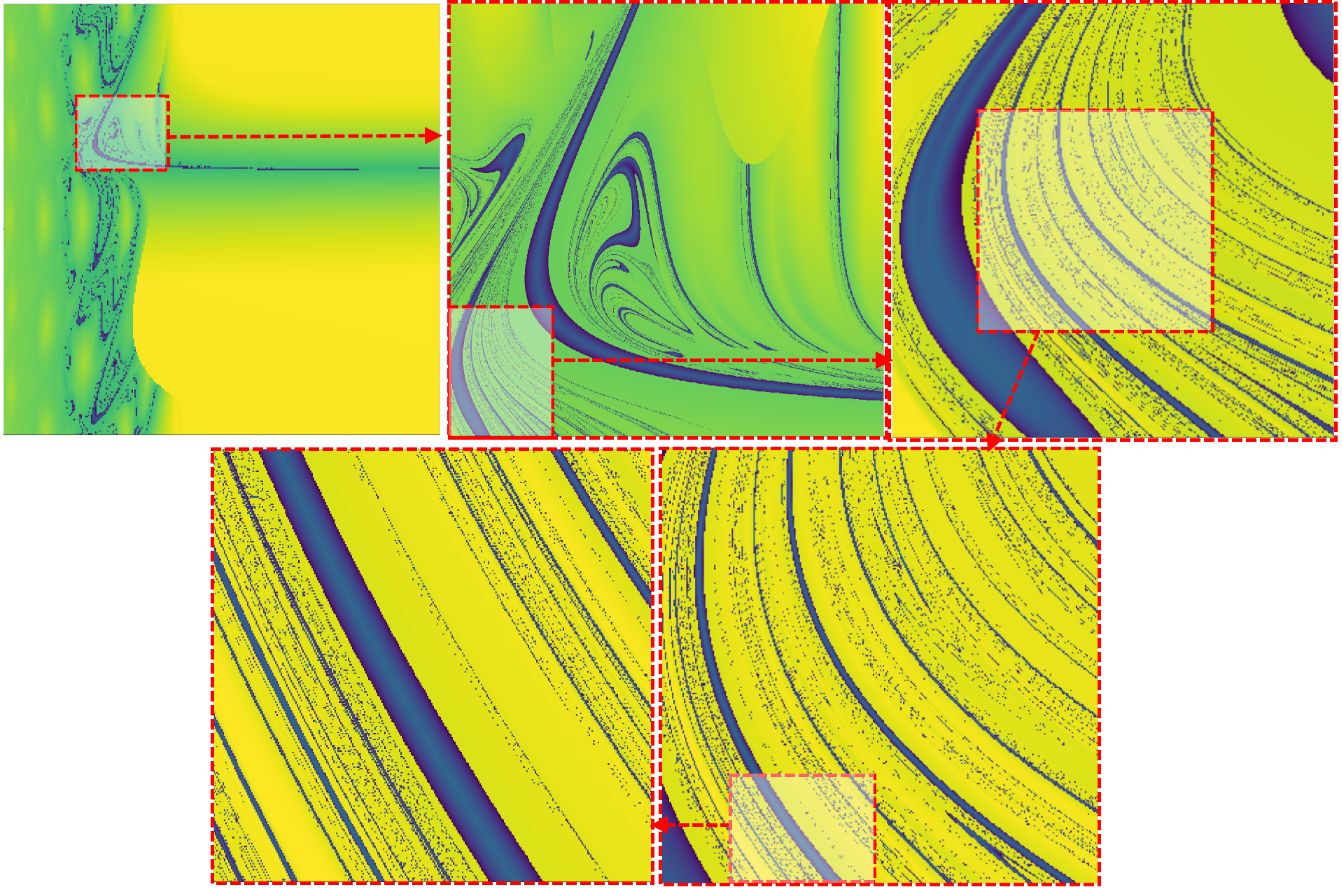
\includegraphics[width=\linewidth]{fig/consecutivezoom.png}
    \caption{Repeated zoom-ins on the problem space show regions of fractal ridges, all but necessitating some adaptive variance measure. }
    \label{fig:consecutivezoom}
\end{figure} 

\begin{figure}
    \centering
    \subfloat[Optimization path]{
        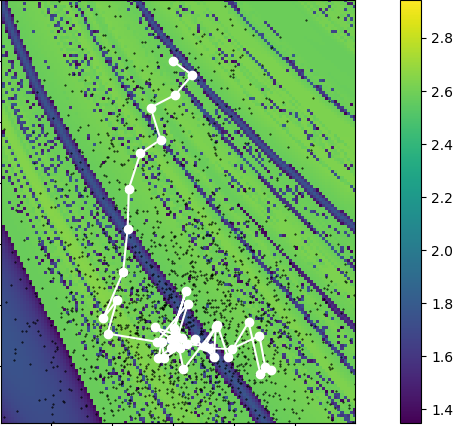
\includegraphics[width=0.46\linewidth]{fig/confusioninfractalarea}
        \label{fig:confusioninfractalarea}
    }
    \hfill
    \subfloat[current (red), best (black), and average (blue) score at each iteration]{
        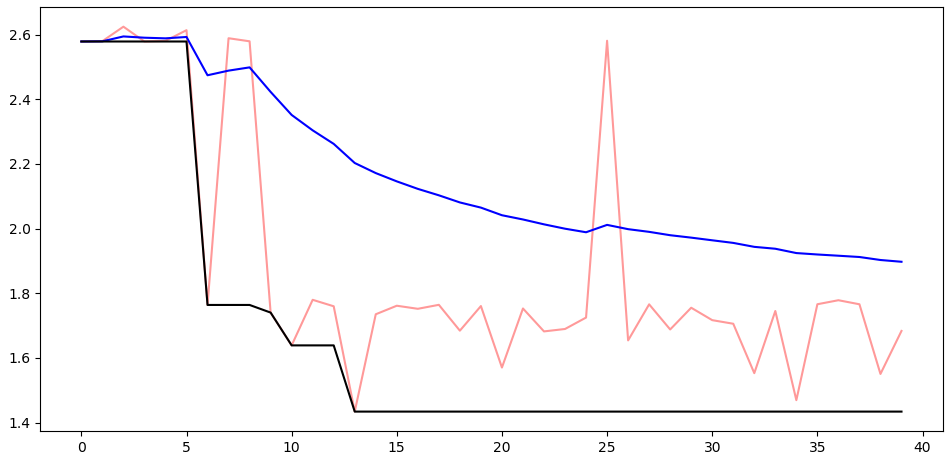
\includegraphics[width=0.46\linewidth]{fig/confusioninfractalarea_scoreplot}
        \label{fig:confusioninfractalarea_scoreplot}
    }
    \caption{The algorithm experiences confusion when it starts in a fractal area}
\end{figure}
\begin{figure}[ht]
    \subfloat[Optimization path]{
        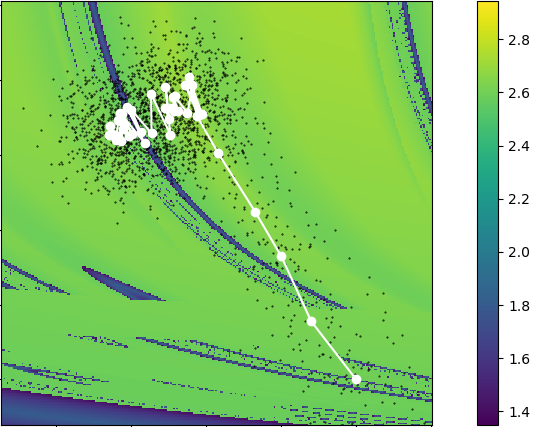
\includegraphics[width=0.46\linewidth]{fig/findingridge.PNG}
        \label{fig:findingridge}
    }
    \hfill
    \subfloat[current (red), best (black), and average (blue) score at each iteration]{
        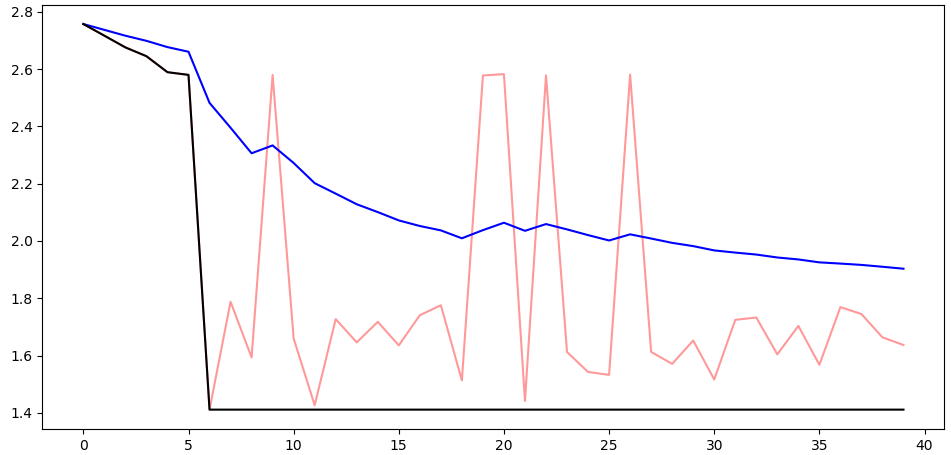
\includegraphics[width=0.46\linewidth]{fig/findingridge_scoreplot}
        \label{fig:findingridge_scoreplot}
    }
    \caption{Here we see the algorithm locating and settling in a ridge}
\end{figure}
\begin{figure}[ht]
    \subfloat[Optimization path]{
        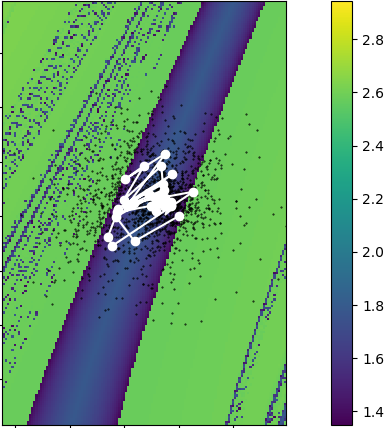
\includegraphics[width=0.46\linewidth]{fig/chilling_on_ridge.png}
        \label{fig:chilling_on_ridge}
    }
    \hfill
    \subfloat[current (red), best (black), and average (blue) score at each iteration]{
        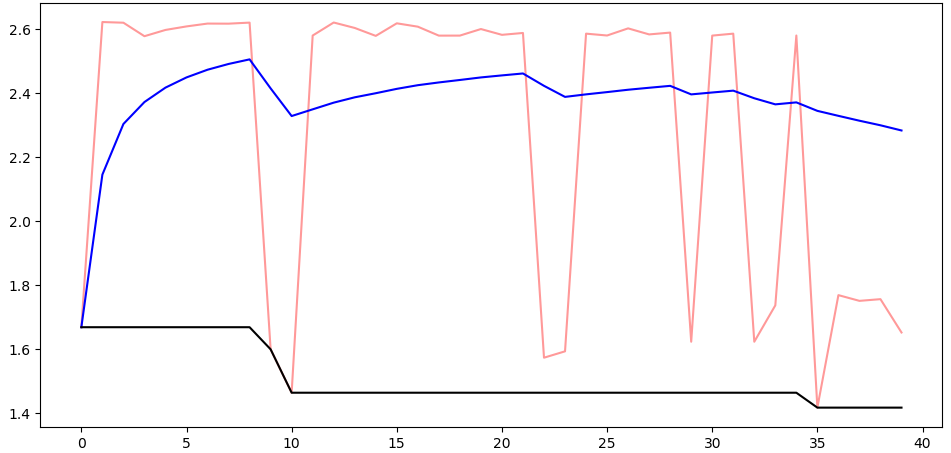
\includegraphics[width=0.46\linewidth]{fig/chilling_scoreplot}
        \label{fig:chilling_scoreplot}
    }
    \caption{We see that there is not much of a gradient along the ridges. This might indicate that a momentum-based strategy might be a valuable addition, if we want to search the ridges properly. CMA-ES is also an interesting prospect, for the same reason.}
\end{figure}
\begin{figure}[ht]
    \subfloat[Optimization path nicely finding a ridge and staying on it.]{
        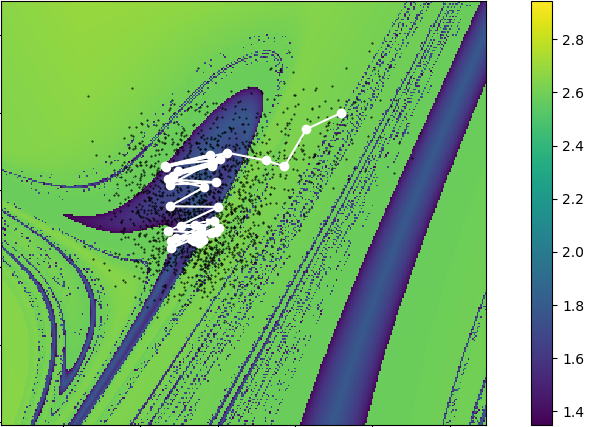
\includegraphics[width=0.46\linewidth]{fig/EScatchingridge.png}
        \label{fig:EScatchingridge}
    }
    \hfill
    \subfloat[current (red), best (black), and average (blue) score at each iteration]{
        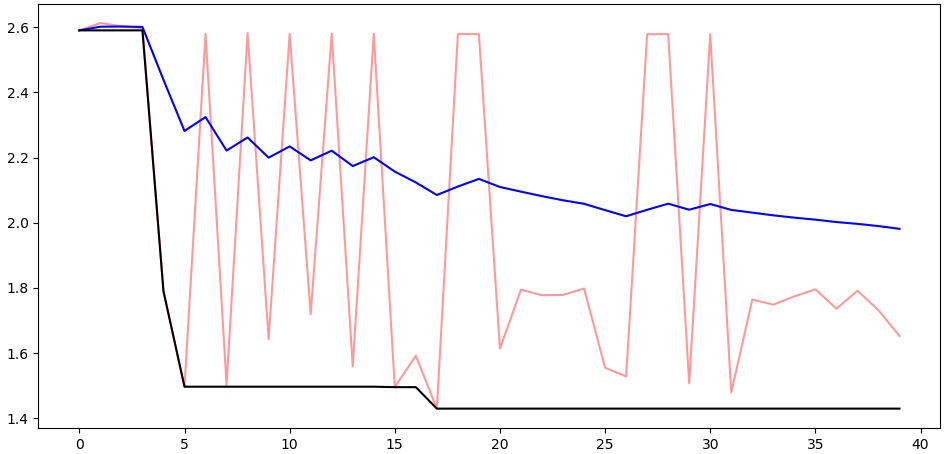
\includegraphics[width=0.46\linewidth]{fig/EScatchingridge_scoreplot}
        \label{fig:EScatchingridge_scoreplot}
    }
    \caption{Various examples of the ES algorithm acting from different starting points. A linear variance reduction scheme is present in \cref{fig:chilling_on_ridge}, to gauge the impact of a true variational optimization measure.}
    \label{fig:ES-examples} 
\end{figure} 

\begin{figure}[ht]
    \centering
    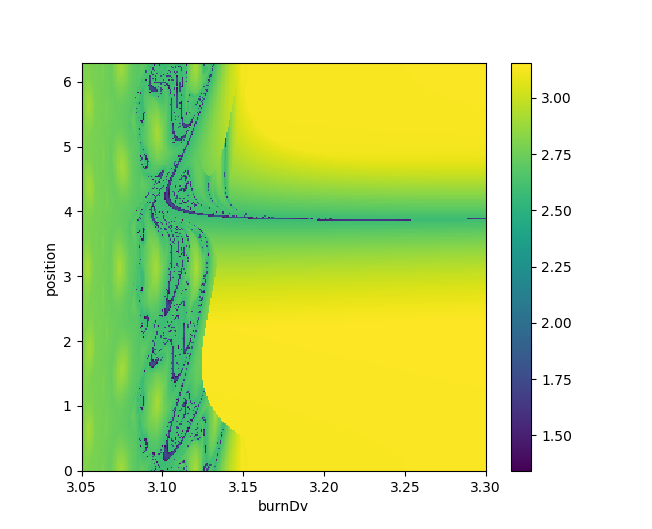
\includegraphics[width=0.7\linewidth]{fig/golf_course_wide.png}
    \caption{The problem space with the bounds that we tried initially: full circle of starting angles, and a much more liberal range of initial burn vector magnitudes. At $burn \Delta v \leq 3.08$ we don't escape from earth, and at $burn \Delta v \geq 3.15$ we simply escape the earth-moon system entirely, apart from the case where we strike the moon directly. The blue line that cuts through the yellow is broadly speaking the class of Hohmann transfers at greater and greater speed. They are not very interesting, so we limited the search bounds for our experiments to what you see in \cref{fig:golf_course_s1024}}
    \label{fig:golf_course_wide}
\end{figure}

\subsection{Comparison with Baseline}
Comparing the ES algorithm with a random guessing baseline, we do not get very encouraging results \cref{fig:randomguessingufig}. Given the parameter bounds used in these experiments (which we believe are quite reasonable given the overall picture of the optimization space \cref{fig:golf_course_wide}), it seems that the space is sufficiently dense with good solutions (that are more or less equally good), that random guessing performs decently. Assuming that the best solutions are found by traversing a ridge, ES still has value, but from what we have seen, the along-ridge gradient is very low.


\begin{figure}[ht]
    \subfloat[Random guessing with 2000 fitness evaluations]{
        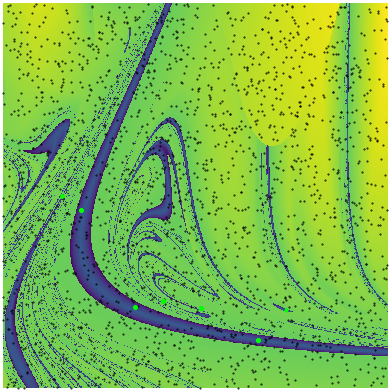
\includegraphics[width=0.46\linewidth]{fig/randomguessing.png}
        \label{fig:randomguessing}
    }
    \hfill
    \subfloat[current (red), best (black), and average (blue) score at each iteration]{
        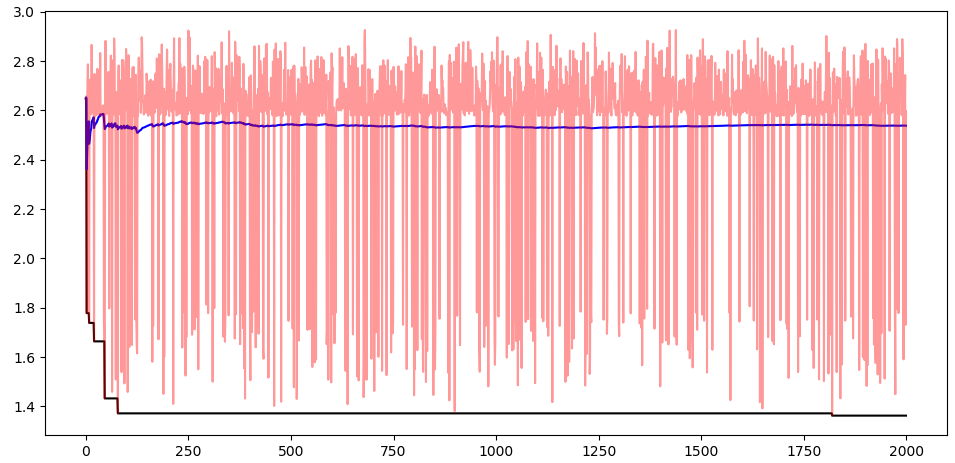
\includegraphics[width=0.46\linewidth]{fig/randomguessing_scoreplot}
        \label{fig:randomguessing_scoreplot}
    }
    \caption{We tried an approach of random guessing, with an equal fitness evaluation budget to the integer valued ES runs (2000). Clearly, random guessing performs very well when looking for decent solutions, since the space is pretty dense with them in 2D, and with these bounds. The average solution found is worse, so there is perhaps still an argument to be made for ES, even at this scale.}
    \label{fig:randomguessingufig} 
\end{figure} 

\section{Real-valued ES algorithm}
The algorithm that generated the problem space plots seen throughout this work has been working with a pre-computed grid of fitness values (\cref{fig:golf_course_s1024}). It's of relatively high resolution, but in a fractal space, any fixed resolution is too low. For that reason, we also maintain a real-value version of the algorithm that works in the full, original 3-dimensional problem space. It runs on the GPU optimized C-version of the Moon-mission simulator (\cref{fig:software_architecture}), and runs the algorithm truly at scale. It does not, however, give us results as nice as the ones we see from the graphical ES algorithm. A selection of scores from this model can be seen in \cref{fig:GPUresults}. There are thousands of these patterns, where the algorithm strikes upon a good solution once in a while, but they are not very interesting, and hard to communicate visually. The difficulty in examining the results en masse make it hard to figure out why we see this difference. As it is now, it looks eerily similar to the performance of random guessing.

\begin{figure}[ht]
    \centering
    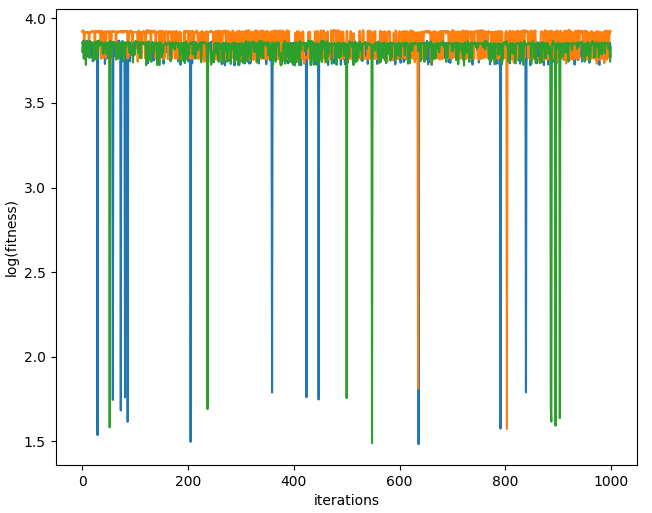
\includegraphics[width=0.6\linewidth]{fig/GPUresults.png}
    \caption{log-fitness score of selected individuals as they evolve through the Real-valued GPU-version of the algorithm. There are thousands more graphs like these, but they all look similarly uninteresting. The difference may be due to the additional degree of freedom in this version of the algorithm.}
    \label{fig:GPUresults}
\end{figure}

\clearpage

\section{3D Simulator: Finding LETOs to Mars}
The 3D simulator based on a spherical coordinate system turned out to be a much more difficult project than anticipated:

\begin{enumerate}
	\item \textbf{The equations of motion turned out to be complicated}, as a restricted N-body system based on spherical coordinates turned out to be quite complicated set of equations, making it prone to typing mistakes when writing into code. In fact we spent many weeks trying to find out why it didn't work as planned, until we decided to systematically debug the program by doing unit testing all major equations with Mathematica and Pytest (as described in \cref{sec:unit-testing}).
	\item \textbf{The positions Earth and Mars turned out to be a tricky problem}. The ellipse equations were surprisingly complex and involved solving multiple implicit equations with no closed-form solutions. We opted for looking up the positions in an ephemerides\footnote{A table or data file giving the calculated positions of a celestial object at regular intervals throughout a period.}. We wanted maximum realism in the 3D simulator (hence why we didn't simply do a 2D simulator to Mars), and using a data table was a way to ensure the realism of the data. However the best data we could find was from the NASA Horizons\footnote{\textit{The JPL Horizons On-Line Ephemeris System provides access to key solar system data and flexible production of highly accurate ephemerides for solar system objects. This includes 780,000+ asteroids, 3525 comets, 178 natural satellites, all planets, the Sun, 150 spacecraft, and several dynamical points such as Earth-Sun L1, L2, L4, L5, and system barycenters} - \url{https://ssd.jpl.nasa.gov/?horizons_doc}.} \cite{NASAb}. Furthermore from a software engineering standpoint we wanted to use table data from NASA instead of doing more math modelling and simulation. However at the time we pulled the data we could not get ephemerides with any higher time step than 1 day\footnote{Since then NASA Horizons now support time steps down to 1 hour. Dare we say ``typical'' 🙄}. I.e. we only have 365 positions for Earth in the year, and opted for a simple linear interpolation at all times in between.
	\item \textbf{The initial conditions were hard to determine given our ephemerides constraints}. Setting initial conditions in 3D space with incomplete information also turned out as a bigger challenge than expected. We determined the initial conditions from an estimation of Earth velocity as the difference of position between two days, did calculations involving cross products, centripetal speed, initial delta-v as per \cref{sec:2d-patched-conic,apx:mars-hohmann-derivations} etc. While we could get nice circular orbits around the Sun or Earth in isolation, we crashed into the Earth when orbiting Earth for more than a few hours. Modelling Earth as a point particle went fine, but setting the radius of the Earth as a stop criteria stopped the simulation after at few orbits at most.
\end{enumerate}

Even if we never made it to Mars in the 3D simulator, we did get basic simulation to run. We obtained closed orbits around Earth or Sun stationary and closed orbits around Earth moving, albeit crossing the surface and crashing (\cref{fig:r4b-leo-crash}) unless Earth was modelled as a point particle (\cref{fig:r4b-leo-no-crash}).

\begin{figure}[ht]
    \centering
    \subfloat[Attempted LEO with symplectic Euler and time step size $h=\SI{1}{\second}$, crashing into the Earth after 1h 2m.]{
        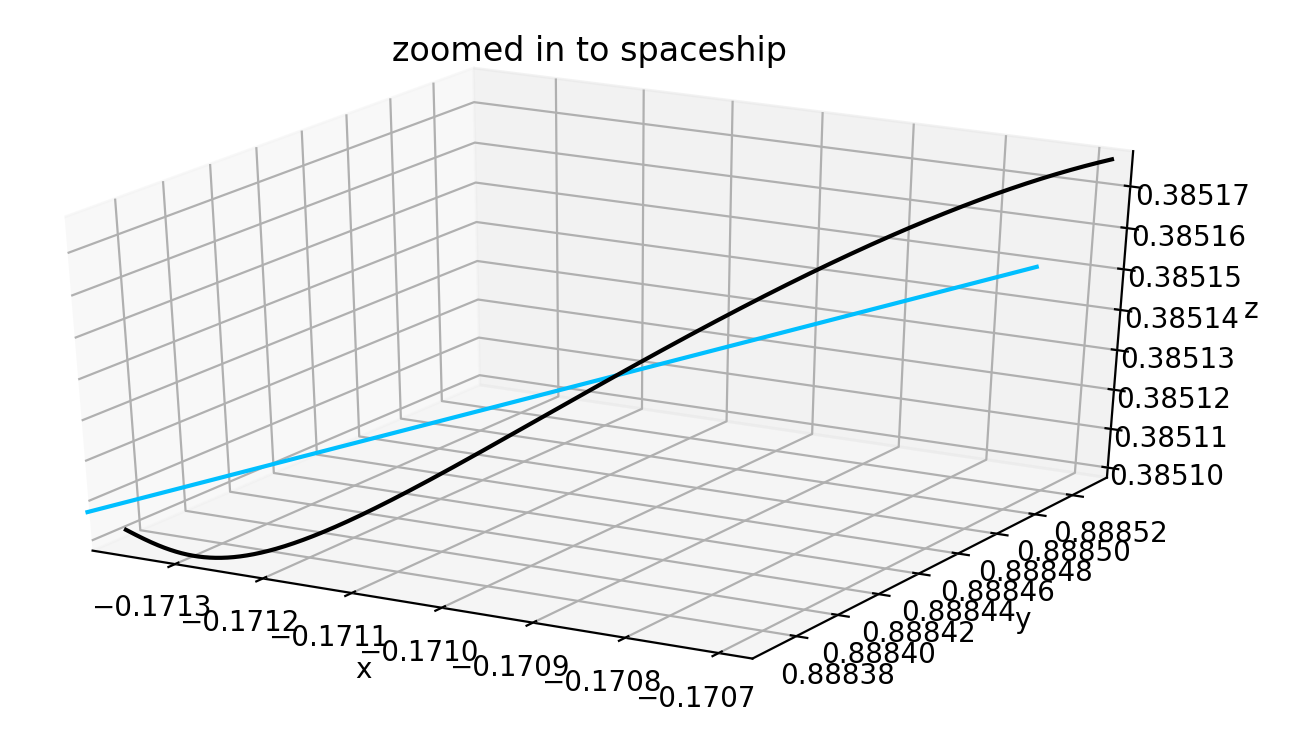
\includegraphics[width=0.45\linewidth]{fig/r4b-leo-crash.png}
        \label{fig:r4b-leo-crash}
    }
    \hfill
    \subfloat[LEO with no Earth crashing logic (Earth as point particle) and $h=\SI{60}{\second}$, clearly showing a closed orbit.]{
        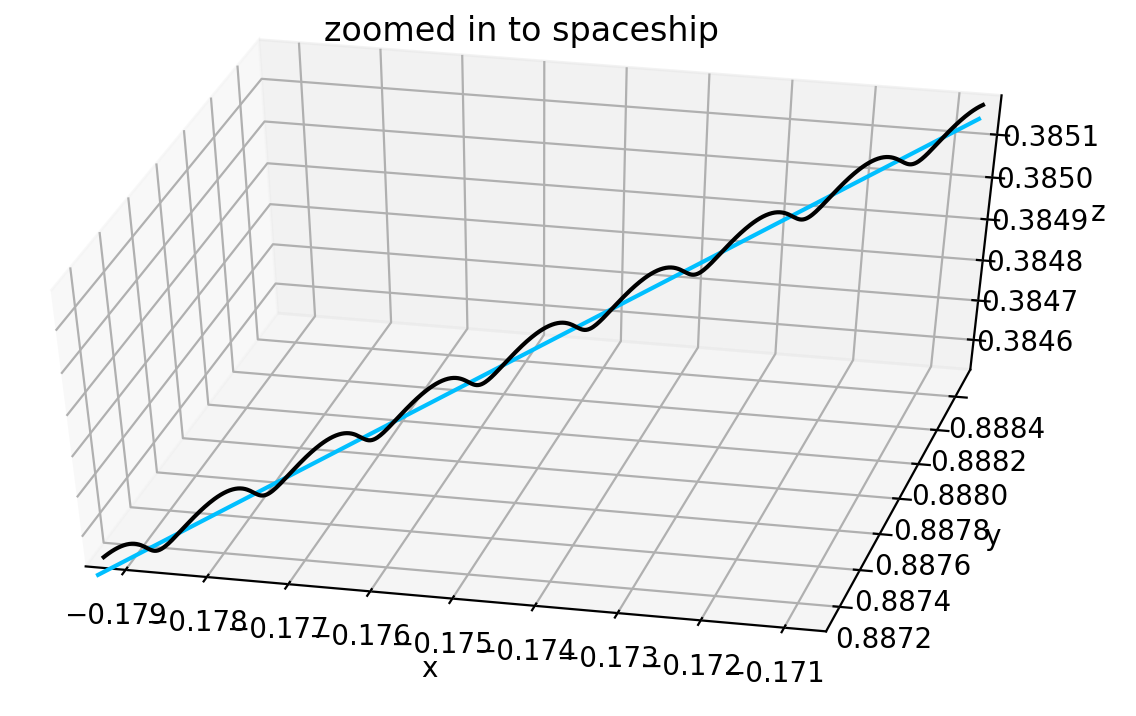
\includegraphics[width=0.45\linewidth]{fig/r4b-leo-no-crash.png}
        \label{fig:r4b-leo-no-crash}
    }
    \caption{Closed orbits around the Earth in the 3D simulator.}
    \label{fig:}
\end{figure} 

We also successfully simulated a run around the sun, see \cref{fig:r4b-sun-orbits}.

\begin{figure}[ht]
    \centering
    \subfloat[Spacecraft, Earth and Mars]{
        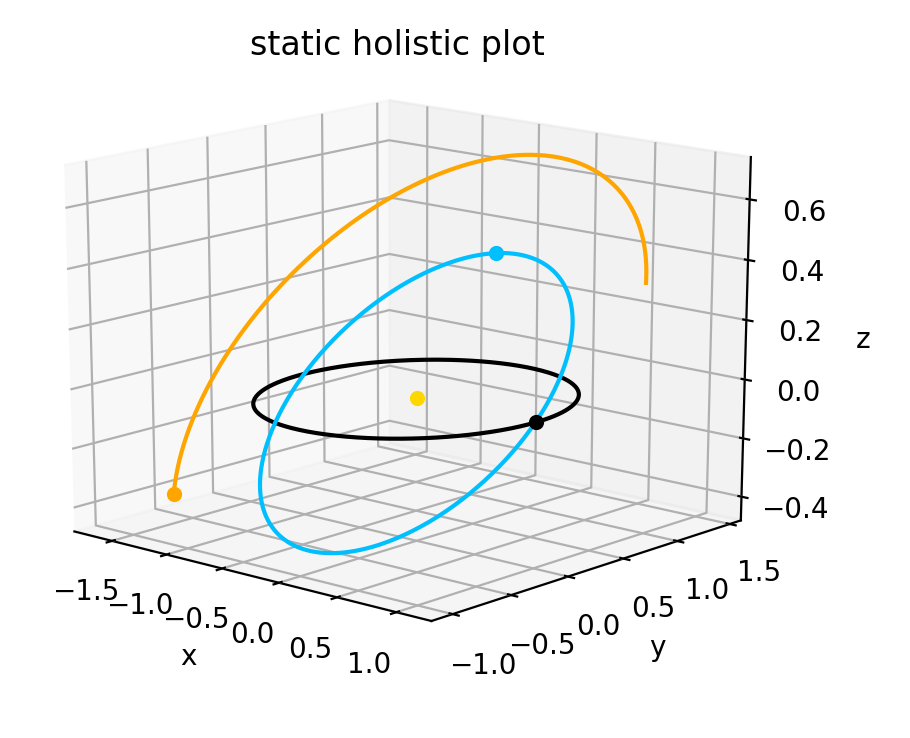
\includegraphics[width=0.30\linewidth]{fig/r4b-sun-orbit.png}
        \label{fig:r4b-sun-orbit}
    }
    \hfill
    \subfloat[Auto-scaled spacecraft orbit to show pertubations from Earth and Mars.]{
        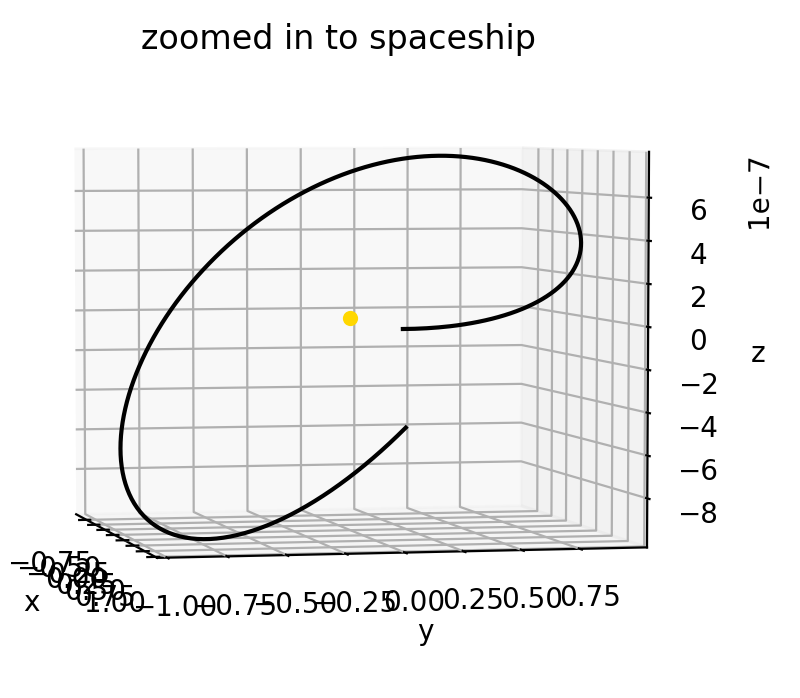
\includegraphics[width=0.30\linewidth]{fig/r4b-sun-orbit-pertubations.png}
        \label{fig:r4b-sun-orbit-pertubations}
    }
    \hfill
    \subfloat[Same as \cref{fig:r4b-sun-orbit-pertubations} but with no pertubations when Earth and Mars masses set to zero.]{
        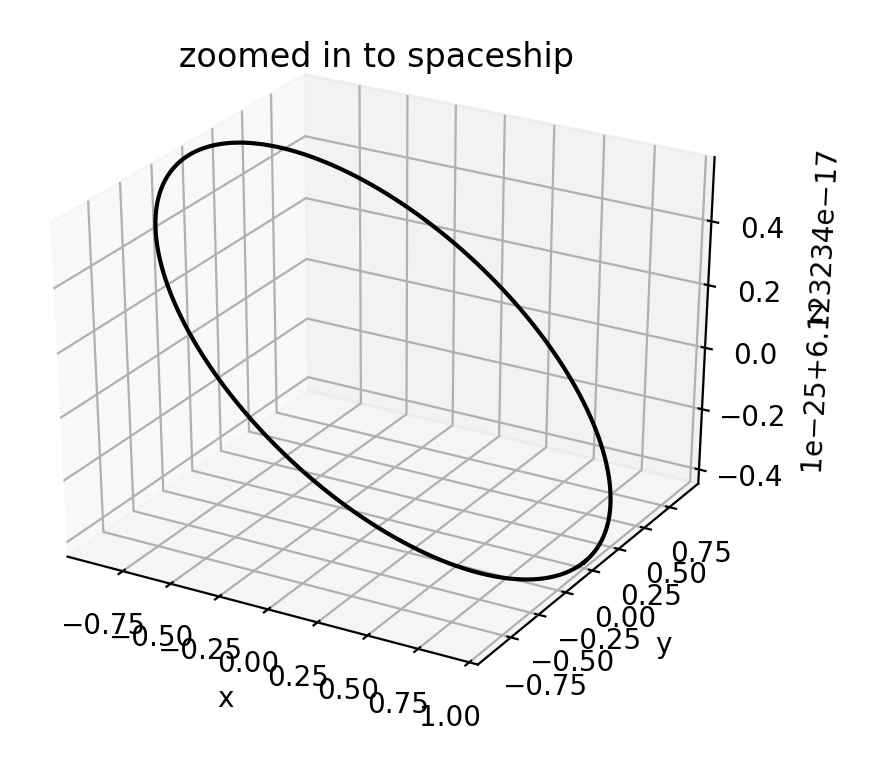
\includegraphics[width=0.30\linewidth]{fig/r4b-sun-orbit-no-pertubations.png}
        \label{fig:r4b-sun-orbit-no-pertubations}
    }
    \caption{Earth in blue orbit in ecliptic plane, spacecraft in orbit in XY-plane, Mars orbit in orange.}
    \label{fig:r4b-sun-orbits}
\end{figure} 

It is clear to us that we were quite close to getting transfer orbits to Mars, especially with the JPL Horizons ephemerides suddenly being available in higher time resolution, which would side-step the linear interpolation issue of the ephemerides. In the end we did get an appreciation of the complexities of working with a simulator in 3D, and it is now obvious to us why much research into LETOs even to Mars are done in 2D (e.g. \cite{Topputo2014}).

\section{Stability of Trajectories: Lyapunov Exponent}
\subsection{Sensitivity analysis}

In our experiments, we found that our paths were diverging pretty heavily given relatively small changes to initial conditions. This was a concern in the original project as well, but was not fully explored then. It is important to quantify the chaotic nature of a system like this, since we are dealing with numerical simulation, which will always have some error associated with it. One takes steps to minimize such errors, often sacrificing computing performance to do so. However, if a system has an error of magnitude say \(\num{1e-8}\), and the system is so chaotic that errors of or \(\num{1e-9}\) at one point early in the trajectory effect meaningful changes further down the line, then the path is near invalid! Therefore, it is important to try to quantify the chaos of a system (in this case our simulator), to provide assurances that the resulting paths have any meaningful truth to them. We have done this by calculating Lyapunov exponents for the system, explained below.

\subsection{Lyapunov Exponent}

The Lyapunov exponent describes the rate of change as time goes on between time series with infinitesimally different starting conditions, as they progress. The method is to compute a set of trajectories, and take the difference between them at set points in time (euclidean distance when dealing with higher dimensions). In a chaotic system, these two trajectories should diverge from each other at some exponential rate, and the Lyapunov exponent is that rate. If we want to trust our results, we want that number to be as low as possible. 

\subsection{Implementation}

We ran several simulations of known good trajectories, with their starting conditions very slightly perturbed, in such a way that the trajectories initially diverged from each other by a value less that 1e-8, chosen as the square root of the precision of the 64-bit floating point numbers that describe the coordinates. The trajectories were then discretized to synchronize the variable length of the time steps, and then compared in pairs, tick by tick, yielding a list of euclidean distances at each step. We then took the natural logarithm of these lists, giving us the plots pictured in \cref{fig:long_leto_slope,fig:hohmann_slope}. The graph varied heavily depending on the gist of the trajectory in question, with trajectories that made multiple passes near earth giving the tooth-like distance graphs pictured in \cref{fig:long_leto_slope}. Trajectories that did not visit earth more than once gave much more `normal' results, given what we see in the literature pertaining to Lyapunov exponent analysis. Clearly, passing into the LEO domain has a powerful stabilizing effect on the the chaotic system, acting like a focal lens for the trajectories passing through. It's not completely trivial to give a Lyapunov exponent from this, but since the individual tooth-segments have a more or less equivalent slope, we simply took the average slope of all the teeth. A deeper look into this cyclical chaos would be interesting, but we will not delve deeper than this.

A good heuristic for whether or not our paths are precise enough would be a measure that would give some confidence interval for final position, given the gist of a trajectory, and the duration of flight along it.

\begin{figure}
    \centering
    \subfloat[A straight-forward Hohmann transfer (yellow-red gradient) and its perturbation (black)]{
        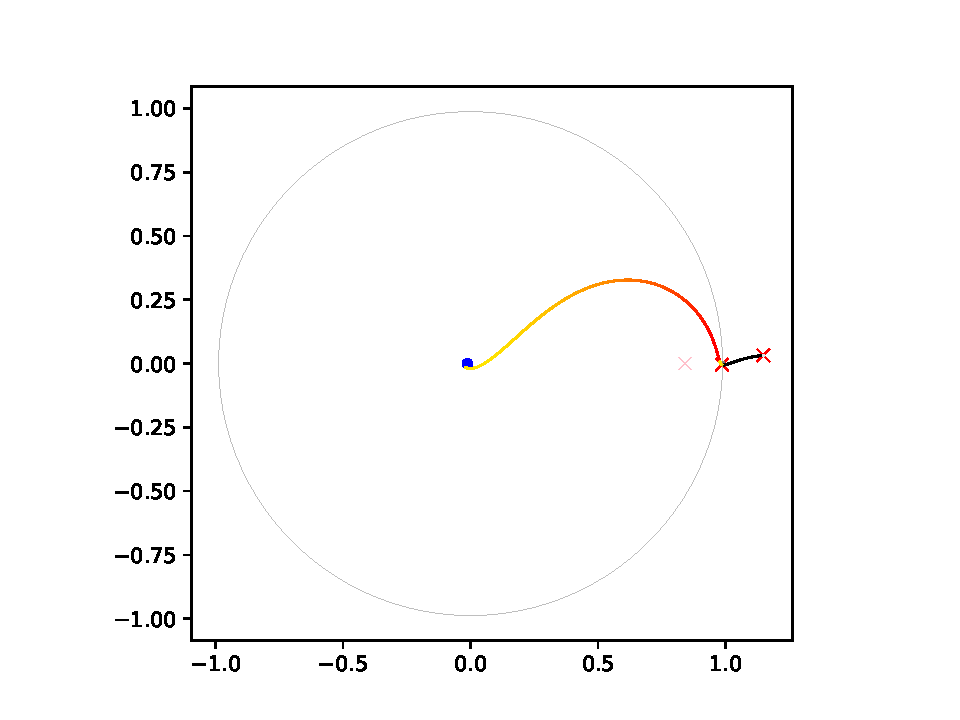
\includegraphics[width=0.46\linewidth]{fig/path_hohmann_nonin_multi_0_and_3.pdf}
        \label{fig:path_hohmann_non-inertial_multi}
    }
    \hfill
    \subfloat[The rate of separation between infinitesimally perturbed versions of the Hohmann transfer]{
        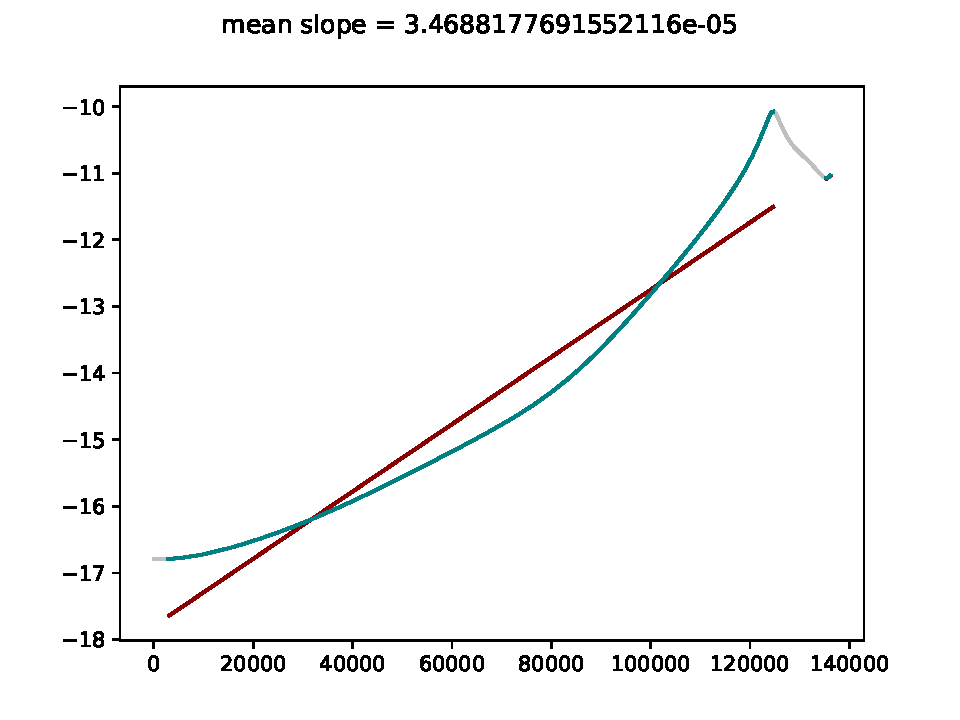
\includegraphics[width=0.46\linewidth]{fig/hohmann_slope_0_and_3}
        \label{fig:hohmann_slope}
    }
    \\
    \subfloat[A relatively long LETO path (black) and its perturbation (yellow-red gradient))]{
        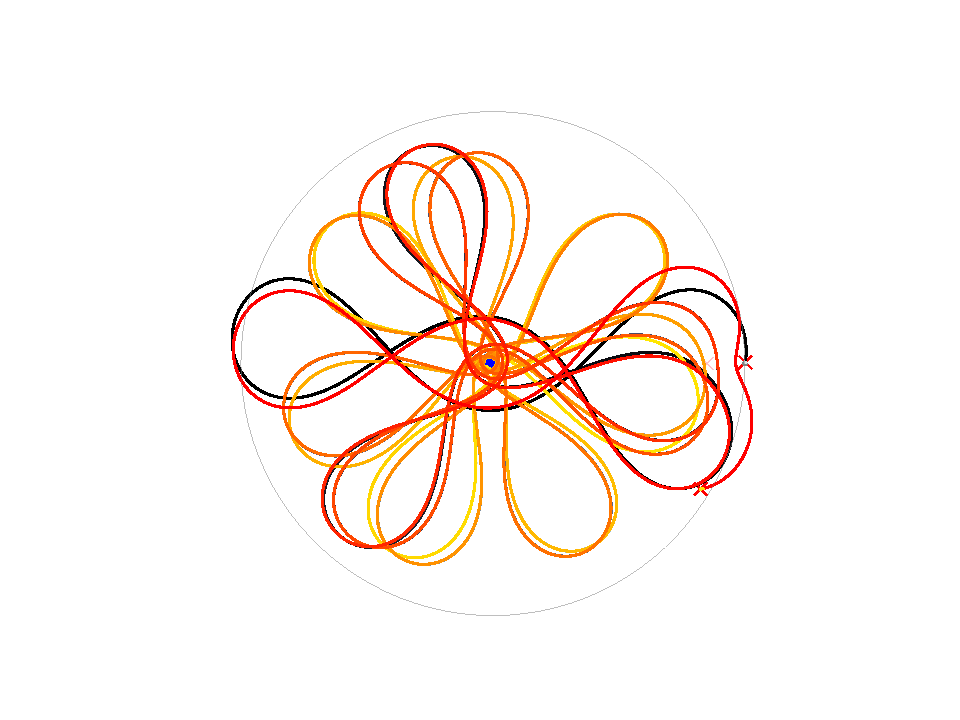
\includegraphics[width=0.46\linewidth]{fig/path_long_leto_nonin_multi_1_and_3.pdf}
        \label{fig:path_long_leto_non-inertial_multi}
    }
    \hfill
    \subfloat[The rate of separation of two infinitesimally perturbed versions of the long LETO]{
        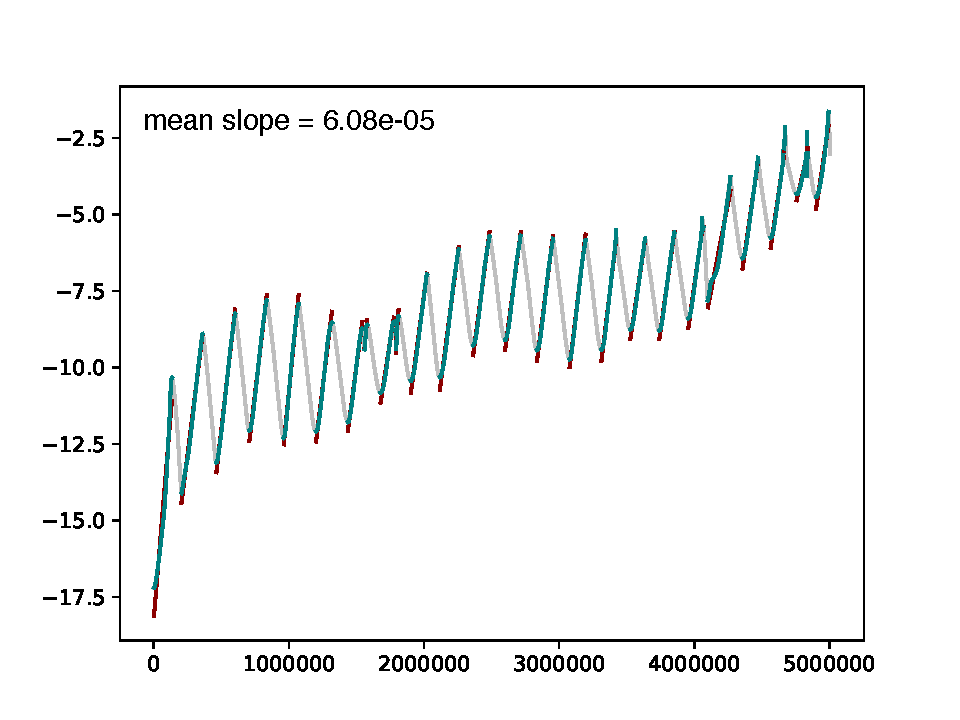
\includegraphics[width=0.46\linewidth]{fig/long_leto_slope_1_and_3}
        \label{fig:long_leto_slope}
    }
    \caption{Examples of some of the different types of transfers that are possible within the model. Each of these were taken as starting points, and simulated again with slightly perturbed starting conditions. The difference between these perturbations were then measured, and plotted in \textbf{b} and \textbf{d}, on a logarithmic scale. The slope of these plots is the lyapunov exponent. We can see that passing into a deep gravity well has a stabilizing effect on the chaos in the system.}
    \label{fig:lyapunov}
\end{figure} 

Our analysis shows that given an initial perturbation in the order of \num{1e-6}, after 200 days we have an uncertainty of 50.000 kilometers. This is a very liberal upper bound for both our error and our flight time. A definite confirmation that the system is significantly chaotic, but not enough to invalidate our results. 

A more reasonable initial perturbation on the order of \num{1e-8} (one order of magnitude greater than our error tolerance) gives us an uncertainty of less than \SI{2700}{km} after the same 200 days (before we pass the moon, which of course stops one path, and heavily diverges the other). This is very manageable for a spacecraft, since it can adjust for these imprecisions with its guidance thrusters early in the process.

The mean slope for our longer and shorter missions remain the same within a single order of magnitude, (\numrange{1e-5}{1e-4}), which is encouraging. Our conclusion with regards to the chaos of the system is that it is significant, and will need to be corrected for dynamically in an actual mission, but that it does not invalidate any trajectories that we find, since the aforementioned dynamic corrections are completely covered by modern- (and to an extent, even vintage) spacecraft capabilities.
